\RequirePackage{fix-cm}
%
\RequirePackage{amsmath}



%\documentclass{svjour3}                     % onecolumn (standard format)
%\documentclass[smallcondensed]{svjour3}     % onecolumn (ditto)
%\documentclass[smallextended]{svjour3}       % onecolumn (second format)
% \documentclass[twocolumn]{svjour3}          % twocolumn
%\documentclass[letterpaper, 12pt, twocolumn]{article}
\documentclass{article}
\usepackage[cm]{fullpage}
%\usepackage[margin=1in]{geometry}
\usepackage{amssymb}
\usepackage{graphicx}
\usepackage[utf8]{inputenc}
\usepackage{indentfirst}
%\usepackage{physics}
\newcommand{\me}{\mathrm{e}}
\usepackage{amsmath}
\usepackage{varwidth}
\usepackage[binary-units]{siunitx}
\usepackage{algpseudocode}
\usepackage{circuitikz}


%\usepackage[monochrome]{color}



%\usepackage[round]{natbib}
%\usepackage{apacite}
\usepackage{url}


\PassOptionsToPackage{monochrome}{xcolor}

% For the flow charts
\usepackage{tikz}
\usetikzlibrary{
	external,
}
\tikzexternalize

\usetikzlibrary{shapes.geometric, arrows, calc, positioning, arrows.meta}
\tikzstyle{startstop} = [rectangle, thick, rounded corners=2.5mm, minimum width=2cm, minimum height=5mm,text centered, draw=black]
\tikzstyle{io} = [trapezium, thick, trapezium left angle=70, trapezium right angle=110, text width=3.75cm, minimum height=0.5cm, text centered, draw=black]
\tikzstyle{process} = [rectangle, thick, minimum width=2.5cm, text width=4cm, minimum height=0.5cm, text centered, draw=black]
\tikzstyle{block} = [rectangle, thick, minimum width=0.5cm, minimum height=1cm, text centered, draw=black]
\tikzstyle{support} = [coordinate, join=by fuzzy]
\tikzstyle{decision} = [diamond, thick, minimum width=3cm, minimum height=1cm, text centered, draw=black]
\tikzstyle{dottedbox} = [rectangle, dotted, thick, minimum width=2.5cm, text width=2.8cm, minimum height=0.5cm, text centered, draw=black]
\tikzstyle{arrow} = [thick,->,>=stealth]
\tikzstyle{dottedarrow} = [thick, dotted,->,>=stealth]
\tikzstyle{FigureArrow} = [-{Stealth[length=3mm, width=2mm]}, line width=0.2mm]




\usepackage{pgfplots}
\usepgfplotslibrary{patchplots}
\pgfplotsset{compat=newest, samples=015} %Set this value to 65 for the final version
%\usepgfplotslibrary{dateplot} 


%\providecommand{\keywords}[1]{\textbf{\textit{Index terms---}} #1}

%\journalname{Journal of Science Education and Technology}

\begin{document}
%\section{Figures}

\begin{figure}
	\centering
	\begin{tikzpicture}[node distance = 10mm, auto]
	\node (Excitation) [align=center] {
		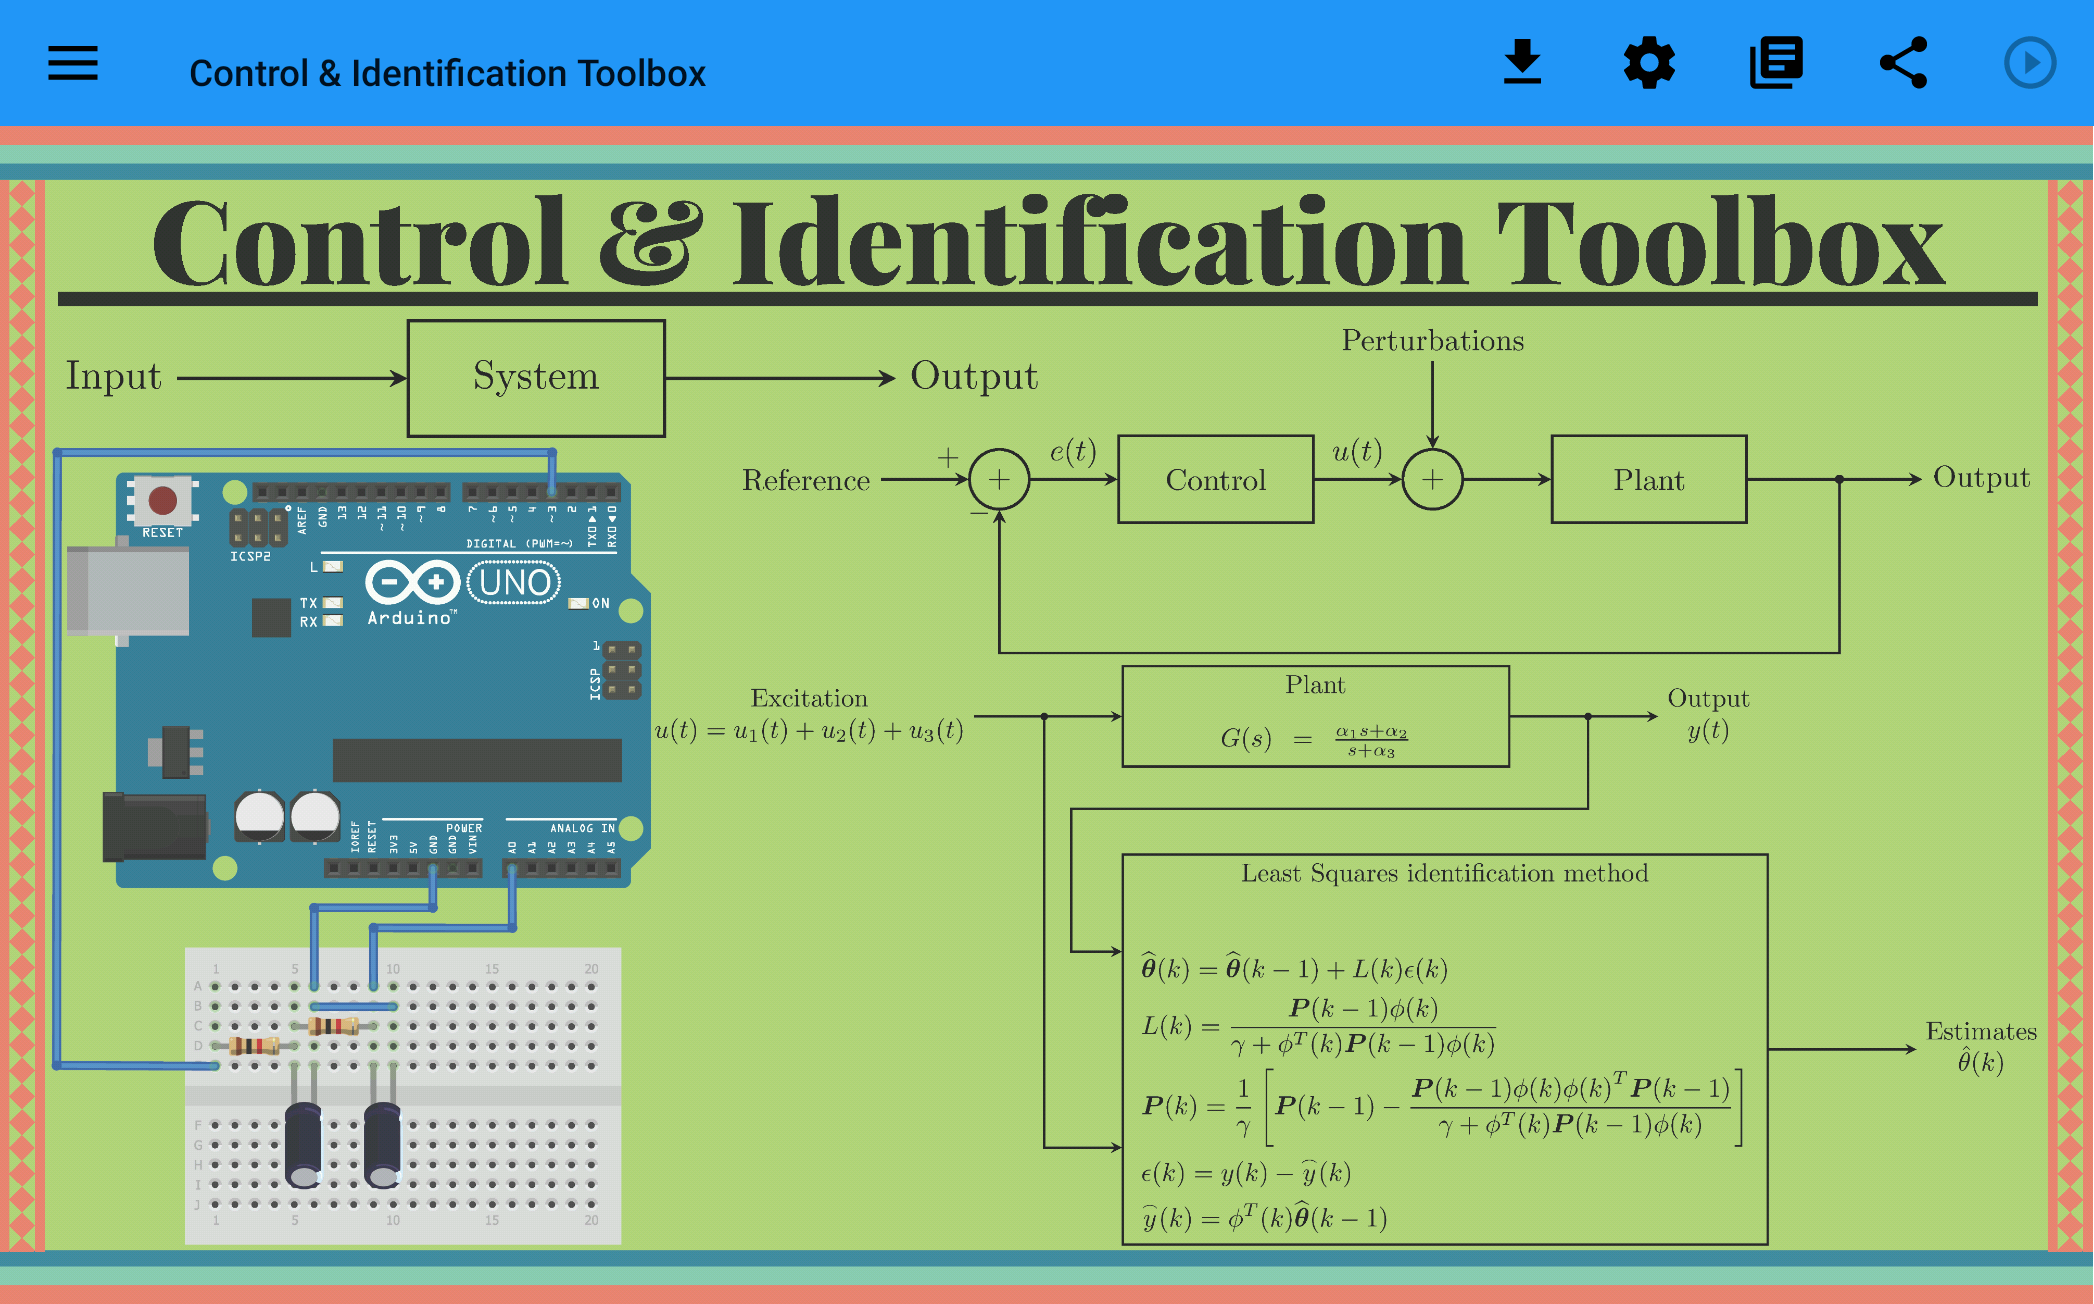
\includegraphics[width=\textwidth]{images/home-screen-color.png}
	};
	\end{tikzpicture}
	\caption{Home-screen of the CIT android application}
	\label{Fig:HomeScreen}
\end{figure}
\begin{figure}
	\centering
	\begin{tikzpicture}[node distance = 10mm, auto]
	\node (Excitation) [align=center] {
		\includegraphics[width=0.5\textwidth]{images/drawer-color.png}
	};
	\end{tikzpicture}
	\caption{Drawer of the CIT android application}
	\label{Fig:Drawer}
\end{figure}
\begin{figure}
	\centering
	\begin{tikzpicture}[node distance = 10mm, auto]
	\node (Excitation) [align=center] {
		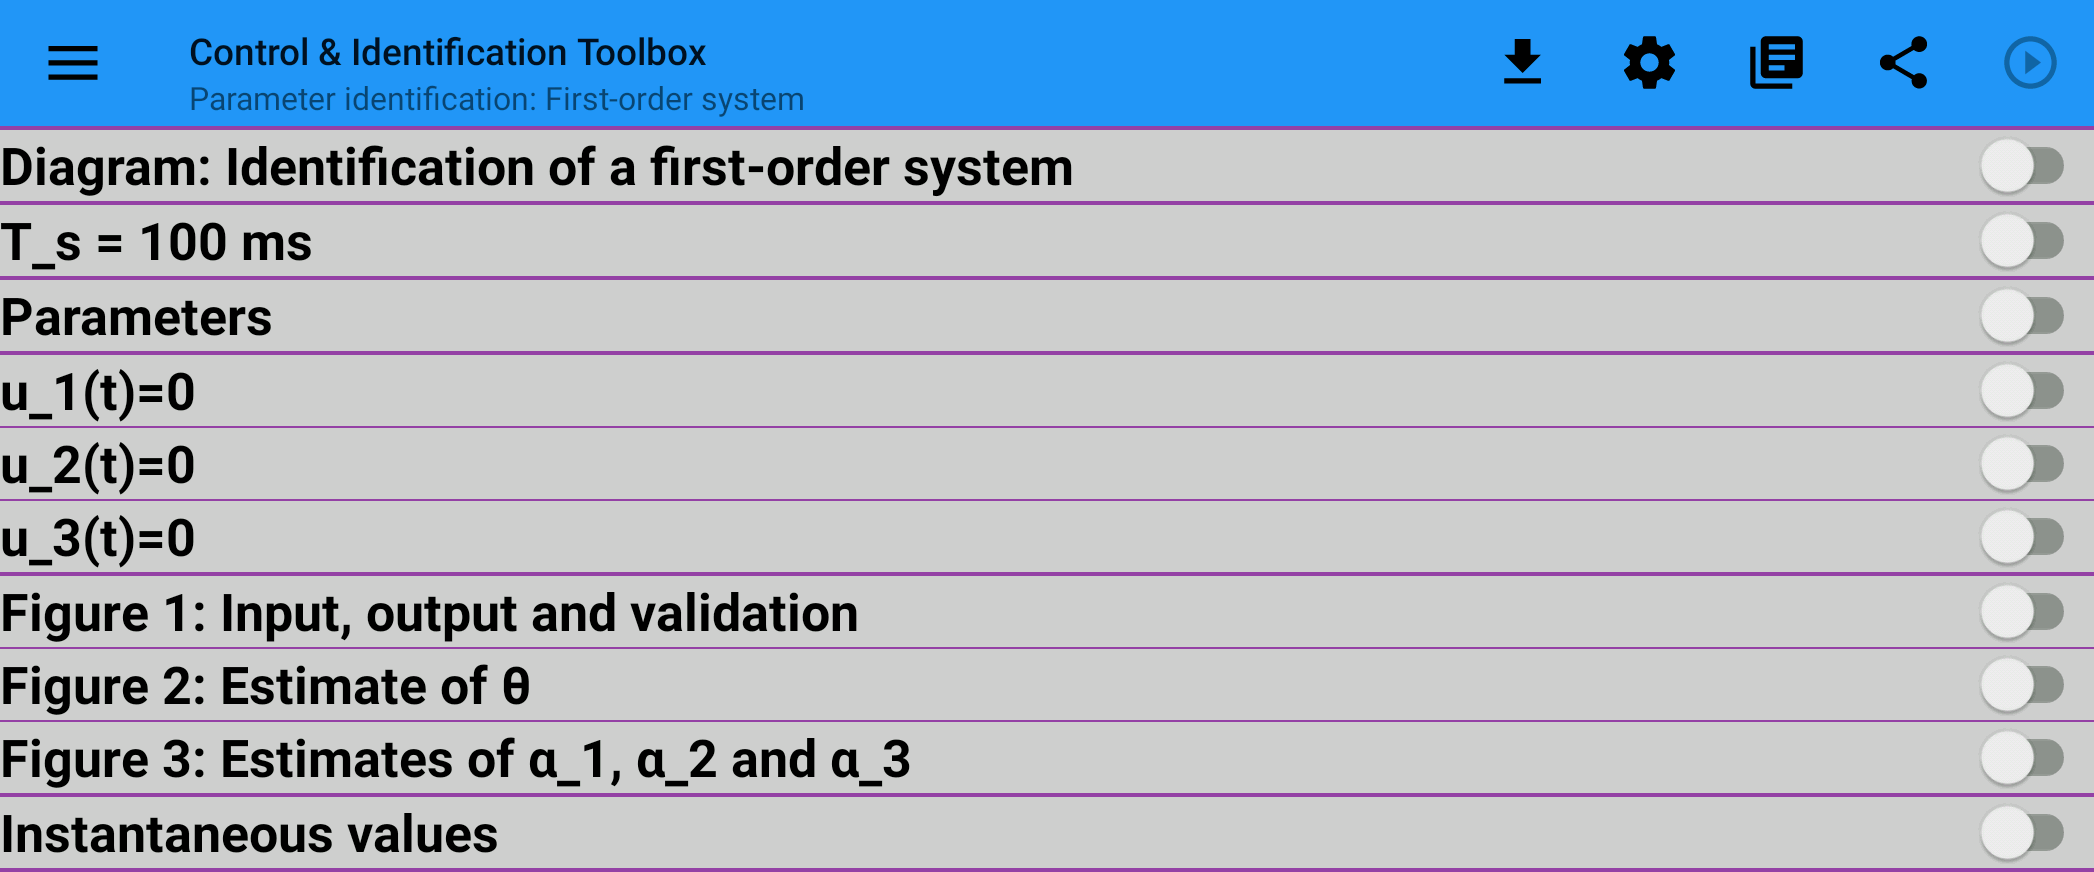
\includegraphics[width=\textwidth]{images/fo-ident-color.png}
	};
	\end{tikzpicture}
	\caption{Experimental results screen (ERS) for first-order parameter identification}
	\label{Fig:FOPIdent}
\end{figure}

\begin{figure}
	\centering
	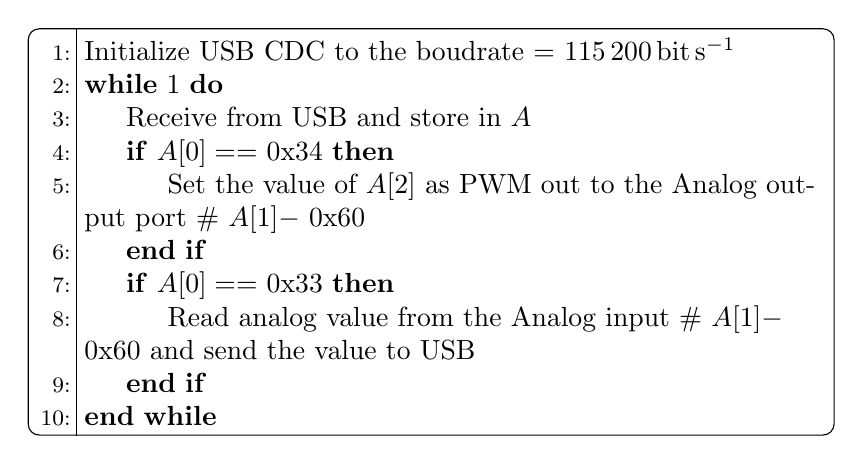
\begin{tikzpicture}[node distance = 10mm, auto]
	\node (algorithm) [draw, rounded corners, text width = 10cm] {% 
		\begin{varwidth}{\linewidth}
		\begin{algorithmic}[1]
		\State Initialize USB CDC to the boudrate = \SI{115200}{\bit\per\second}
		\While {1}
		\State Receive from USB and store in $A$
		\If{$A[0]==$ 0x34}
		\State Set the value of $A[2]$ as PWM out to the Analog output port \# $A[1]-$ 0x60
		\EndIf
		\If{$A[0]==$ 0x33}
		\State Read analog value from the Analog input \# $A[1]-$ 0x60 and send the value to USB
		\EndIf
		\EndWhile
		\end{algorithmic}
		\end{varwidth}
		%
	};
	\draw [-] (algorithm.north)+(-45mm, 0) -- (-45mm,1mm);
	\draw [-] (algorithm.south)+(-45mm, 0) -- (-45mm, 1mm);
	\end{tikzpicture}
	\caption{Bridge device's firmware}
	\label{Fig:Firmware}
\end{figure}

\begin{figure}
	\centering
	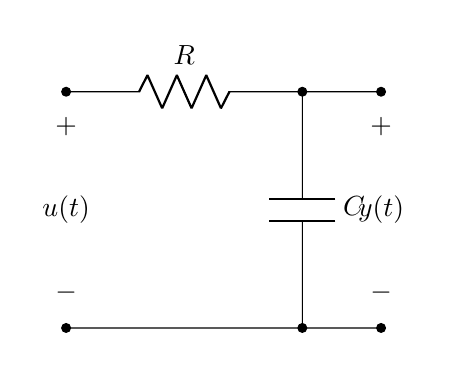
\begin{tikzpicture}[node distance = 10mm, auto]
	\node (Excitation) [align=center] {
		\begin{circuitikz}[american][americanvoltages]
		\draw (0,0)
		to [open, -*, v^<=$u(t)$] (0,3) 
		to[R, -*, l=$R$] (3,3)
		to[C, -*, l=$C$] (3,0)
		to[short, -*] (0,0);
		\draw (3,3)
		to [short, -*] (4,3)
		to [open, -*, v^>=$y(t)$] (4,0)
		to [short] (3,0);
		%		\draw[thin, <-, >=triangle 45] (1,1)node{$i_1$}  ++(-60:0.5) arc (-60:170:0.5);		
		\end{circuitikz}
	};
	\end{tikzpicture}
	\caption{First order low pass filter}
	\label{Fig:CircuitRC1}
\end{figure}

\begin{figure}
	\centering
	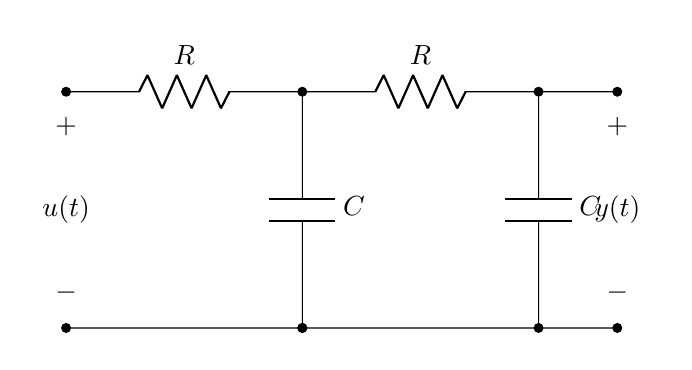
\begin{tikzpicture}[node distance = 10mm, auto]
	\node (Excitation) [align=center] {
		\begin{circuitikz}[american][americanvoltages]
		\draw (0,0)
		to [open, -*, v^<=$u(t)$] (0,3) 
		to[R, -*, l=$R$] (3,3)
		to[C, -*, l=$C$] (3,0)
		to[short, -*] (0,0);
		\draw (3,3)
		to[R, -*, l=$R$] (6,3)
		to[C, -*, l=$C$] (6,0)
		to[short, -*] (3,0);
		\draw (6,3)
		to [short, -*] (7,3)
		to [open, -*, v^>=$y(t)$] (7,0)
		to [short] (6,0);
		\end{circuitikz}
	};
	\end{tikzpicture}
	\caption{Second order low pass filter.}
	\label{Fig:CircuitRC2}
\end{figure}

\begin{figure}
		\centering
	\begin{tikzpicture}[node distance = 10mm, auto]
	\node (Excitation) [align=center] {
	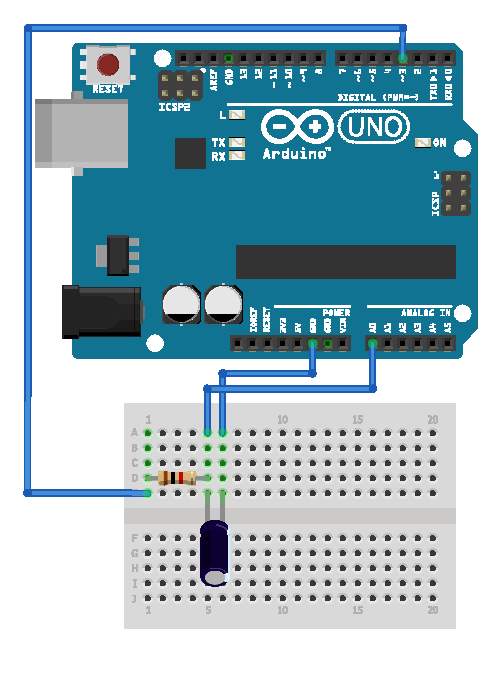
\includegraphics[width=\textwidth]{images/bridge_circuit_first_order_bb-color.pdf}
	};
	\end{tikzpicture}

	\caption{Bridge circuit with a first order RC low pass filter}
	\label{Fig:BridgeCircuit}
\end{figure}

\begin{figure}
	\centering
	\begin{tikzpicture}[node distance = 10mm, auto]
	\node (Excitation) [align=center] {
		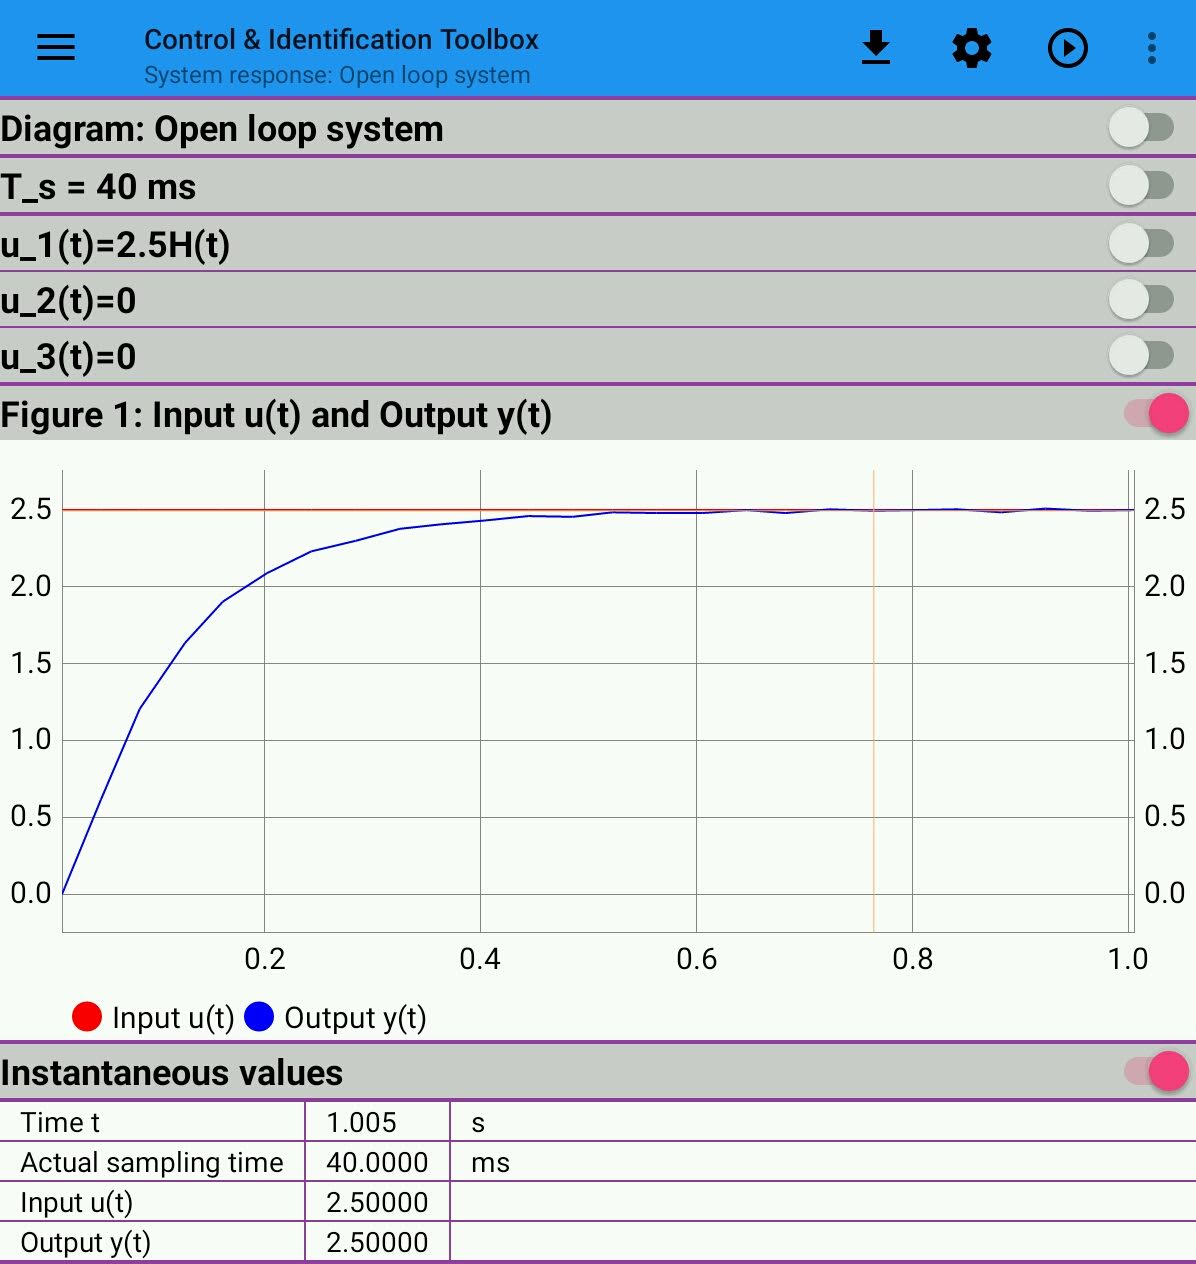
\includegraphics[width=\textwidth]{images/Fig1-color.jpg}
	};
	\draw [FigureArrow] (-4,2.4) node[right] {\Large $u(t)$} -| (-6.3, 1.92);
	\draw [FigureArrow] (-4,0) node[right] {\Large $y(t)$} -- (-6.3, 0);
	\end{tikzpicture}
	
	\caption{Step response of the first-order low pass filter.}
	\label{Fig:SystemResponseStep}
\end{figure}

\begin{figure}
	\centering
	\begin{tikzpicture}[node distance = 10mm, auto]
	\node (Excitation) [align=center] {
		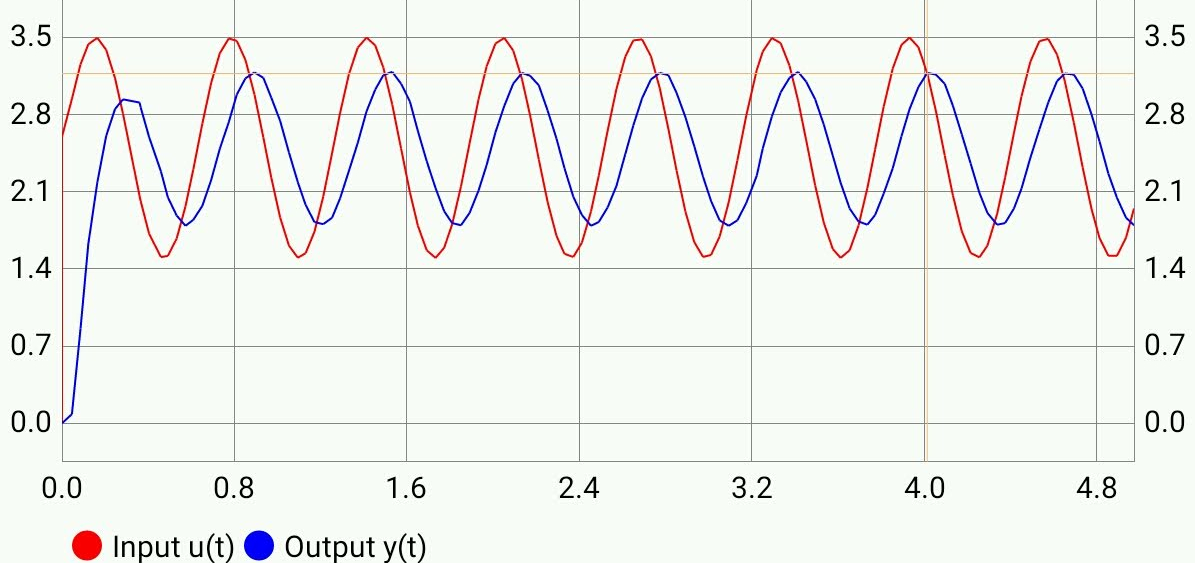
\includegraphics[width=\textwidth]{images/Fig2_cortada-color.jpg}
	};
	\draw [FigureArrow] (-4,-0.5) node[right] {\Large $u(t)$} -| (-6.8, .35);
	\draw [FigureArrow] (-4,-1.5) node[right] {\Large $y(t)$} -- (-8.15, -1.5);
	\end{tikzpicture}
	
	\caption{Sinusoidal response of the fist-order low pass filter.}
	\label{Fig:SystemResponseSine}
\end{figure}

\begin{figure}
	\centering
	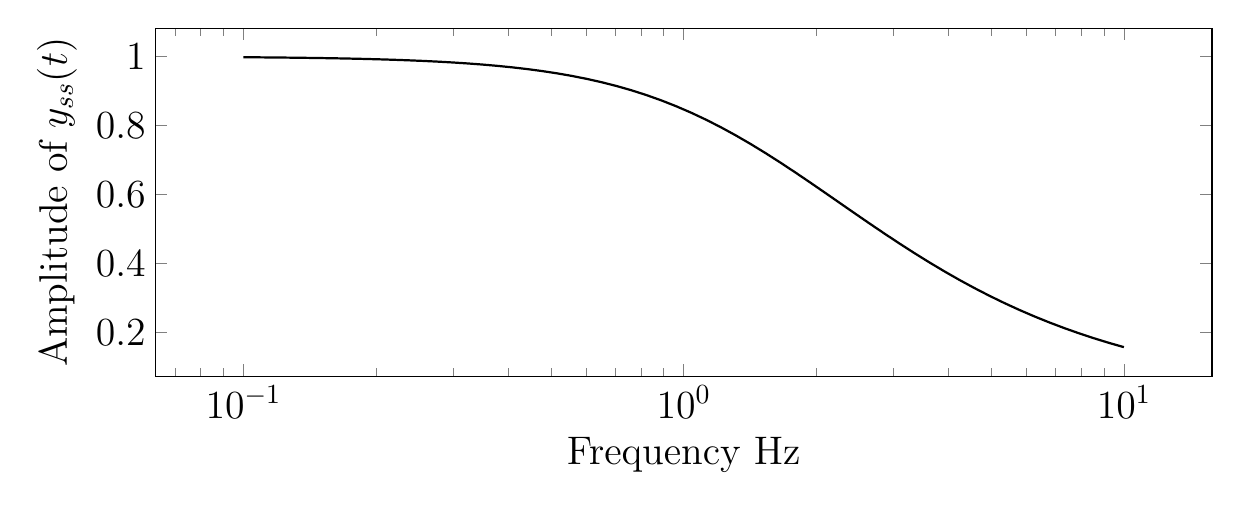
\begin{tikzpicture}
	\begin{axis}[
	font=\Large,
	xmode=log,
	xlabel={Frequency \si{\hertz}},
	width=15cm,
	height=6cm,
	ylabel={Amplitude of $y_{ss}(t)$}
	]
	% use TeX as calculator:
	\addplot [samples=60, domain=0.1:10, thick]{1/(sqrt(1+(2*pi*x/10)^2))};
	\end{axis}
	\end{tikzpicture}
	
	\caption{Magnitude of the frequency response of the first-order low pass filter.}
	\label{Fig:FOFilter}
\end{figure}

\begin{figure}
	\centering
	\begin{tikzpicture}[node distance = 10mm, auto]
	\node (Excitation) [align=center] {
		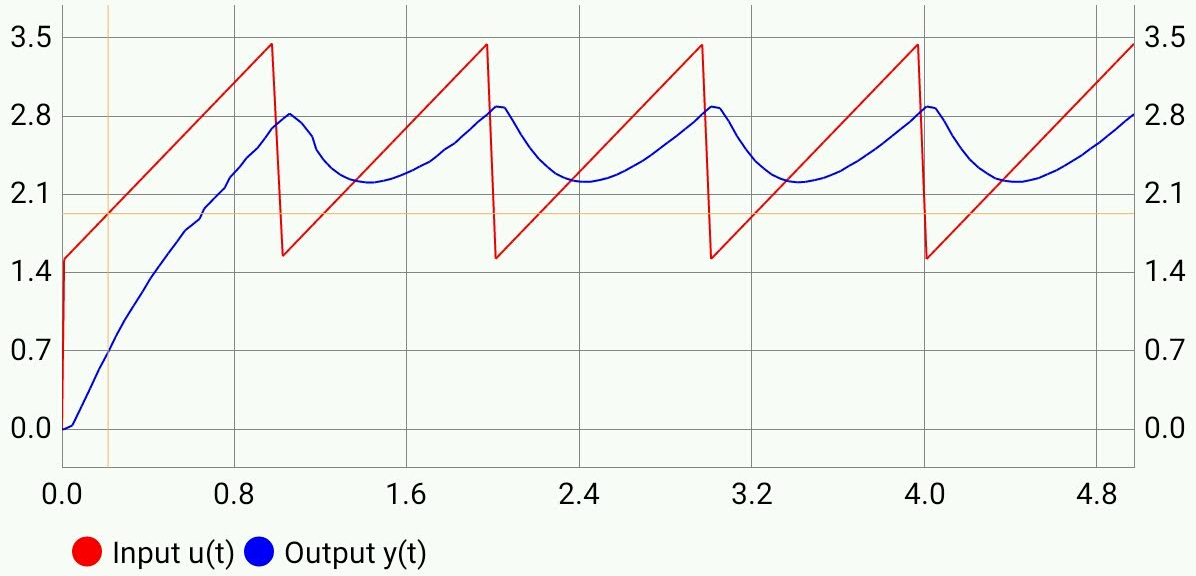
\includegraphics[width=\textwidth]{images/Fig4_cortada-color.jpg}
	};
	\draw [FigureArrow] (-4,-0.5) node[right] {\Large $u(t)$} -| (-4.955, .475);
	\draw [FigureArrow] (-4,-1.5) node[right] {\Large $y(t)$} -- (-7.9, -1.5);
	\end{tikzpicture}
	
	\caption{Response of the second-order filter to a sawtooth wave input.}
	\label{Fig:SystemResponseSawtooth}
\end{figure}

\begin{figure}
	\centering
	\begin{tikzpicture}[node distance = 10mm, auto]
	\node (Excitation) [align=center] {
		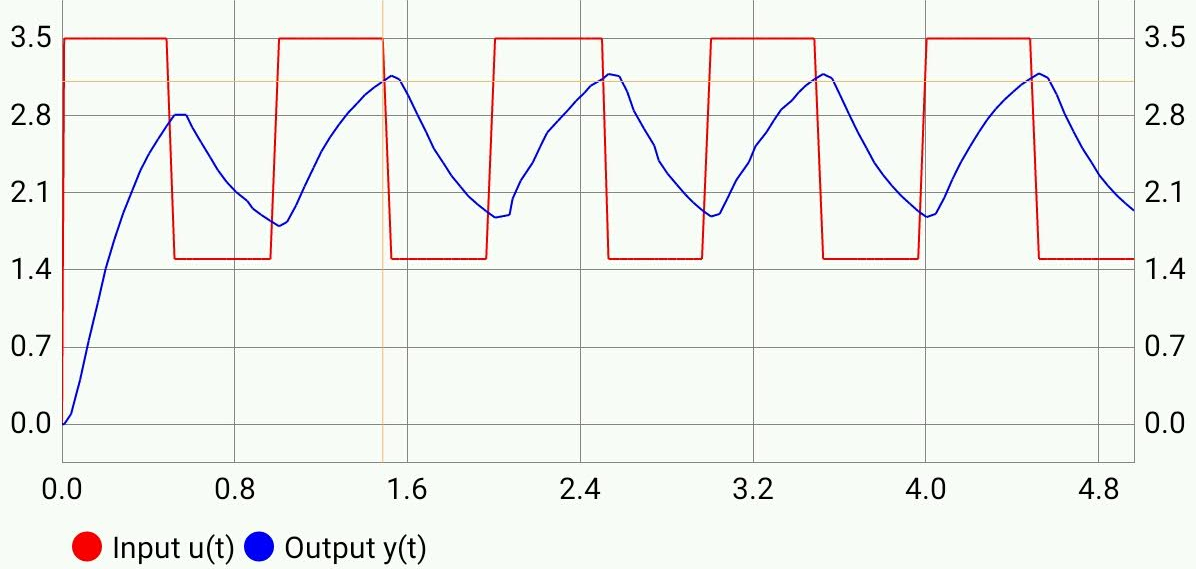
\includegraphics[width=\textwidth]{images/Fig5_cortada-color.jpg}
	};
	\draw [FigureArrow] (-4.5,-0.5) node[right] {\Large $u(t)$} -| (-6, .38);
	\draw [FigureArrow] (-4.5,-1.5) node[right] {\Large $y(t)$} -- (-8.1, -1.5);
	\end{tikzpicture}
	
	\caption{Response of the second-order filter to a square wave input.}
	\label{Fig:SystemResponseSquare}
\end{figure}

\begin{figure}
	\centering
	\begin{tikzpicture}[node distance = 10mm, auto]
	\node (Excitation) [align=center] {
		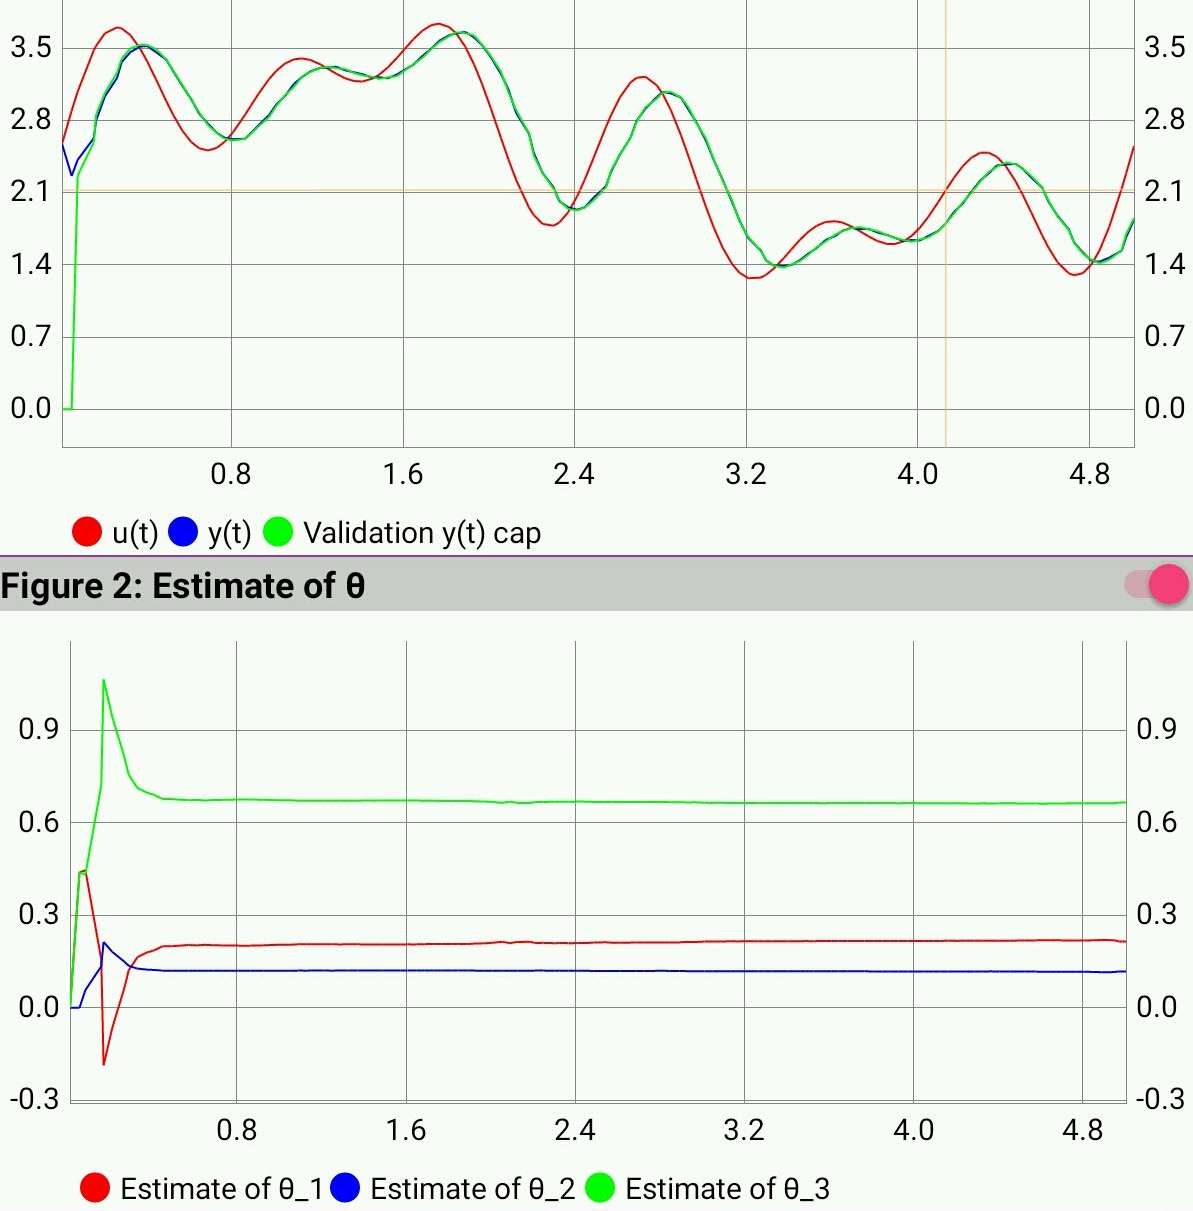
\includegraphics[width=\textwidth]{images/Fig6a-color.jpg}
	};
	\draw [FigureArrow] (-4.5,6) node[right] {\Large $u(t)$} -| (-6.1, 7.075);
	\draw [FigureArrow] (-4.5,4.75) node[right] {\Large $y(t)$} -| (-8.25, 6.7);
	\draw [FigureArrow] (-4.5,3.5) node[right] {\Large $\hat{y}(t)$} -- (-8.2, 3.5);
	\draw [FigureArrow] (-4.5,-7) node[right] {\Large $\hat\theta_1(t)$} -- (-7.67, -7);
	\draw [FigureArrow] (-4.5,-4.25) node[right] {\Large $\hat\theta_2(t)$} -| (-7.5, -5.47);
	\draw [FigureArrow] (-4.5,-1.5) node[right] {\Large $\hat\theta_3(t)$} -- (-7.65, -1.5);
	\end{tikzpicture}
	
	\caption{Signals $u(k)$, $y(k)$, $\hat{y}(k)$ and parameters $\hat{\theta}_{1}$, $\hat{\theta}_{2}$, $\hat{\theta}_{3}$.}
	\label{Fig:FOPA_A}
\end{figure}

\begin{figure}
	\centering
	\begin{tikzpicture}[node distance = 10mm, auto]
	\node (Excitation) [align=center] {
		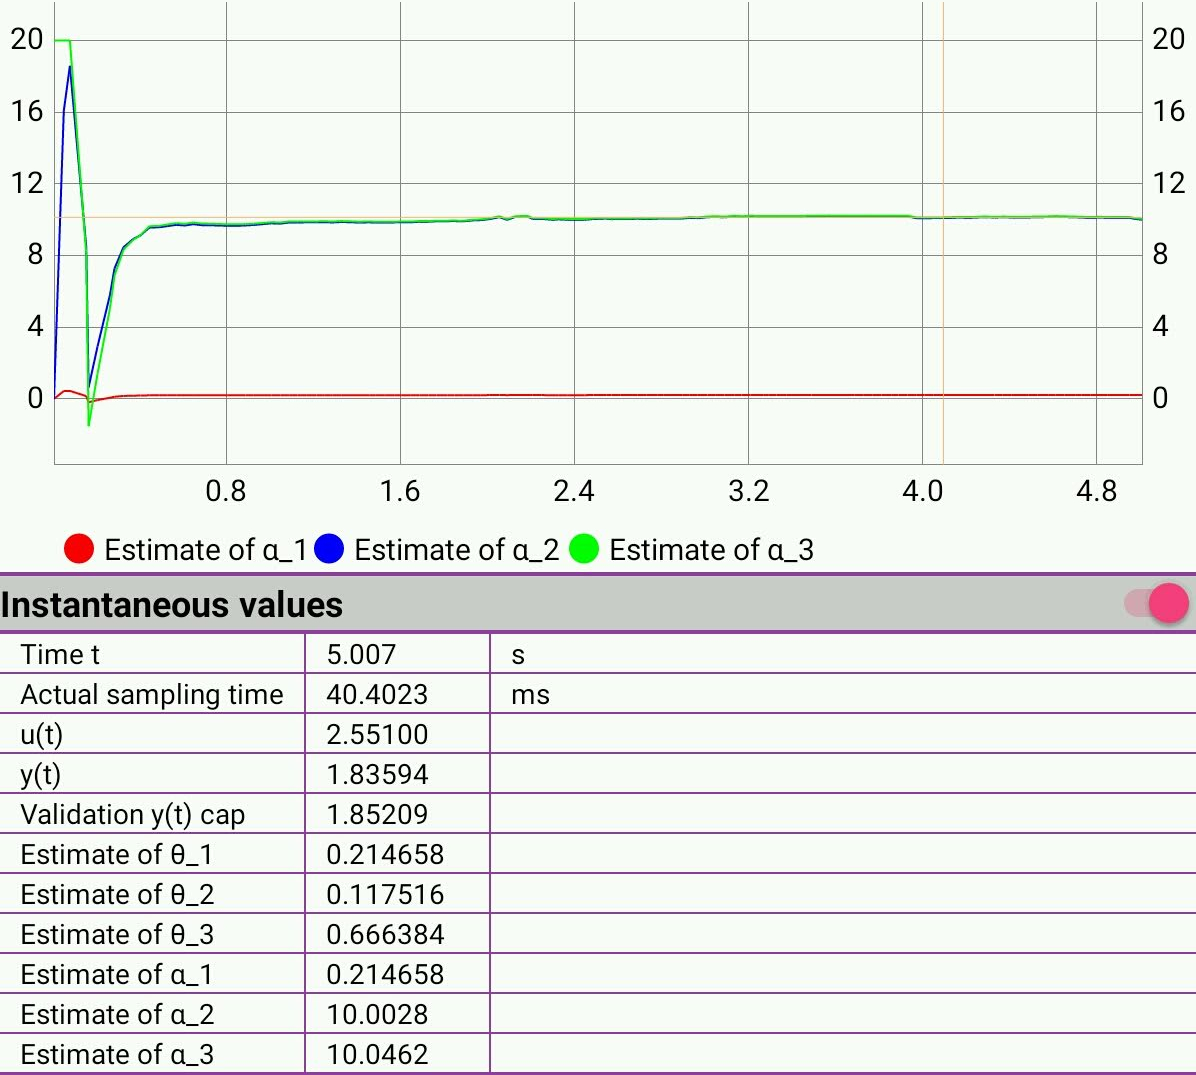
\includegraphics[width=\textwidth]{images/Fig6b-color.jpg}
	};
	\draw [FigureArrow] (-4.5,5.8) node[right] {\Large $\hat\alpha_2$} -- (-8.375, 5.8);
	\draw [FigureArrow] (-4.5,3.8) node[right] {\Large $\hat\alpha_1$} -| (-6, 2.25);
	\draw [FigureArrow] (-4.5,1.8) node[right] {\Large $\hat\alpha_3$} -- (-7.95, 1.8);
	\end{tikzpicture}
	
	\caption{Estimates ${{\hat{\alpha }}_{1}}(t)$, ${{\hat{\alpha }}_{2}}(t)$, ${{\hat{\alpha }}_{3}}(t)$, .and instantaneous values of signals and parameters.}
	\label{Fig:FOPA_B}
\end{figure}

\begin{figure}
	\centering
	\begin{tikzpicture}[node distance = 10mm, auto]
	\node (Excitation) [align=center] {
		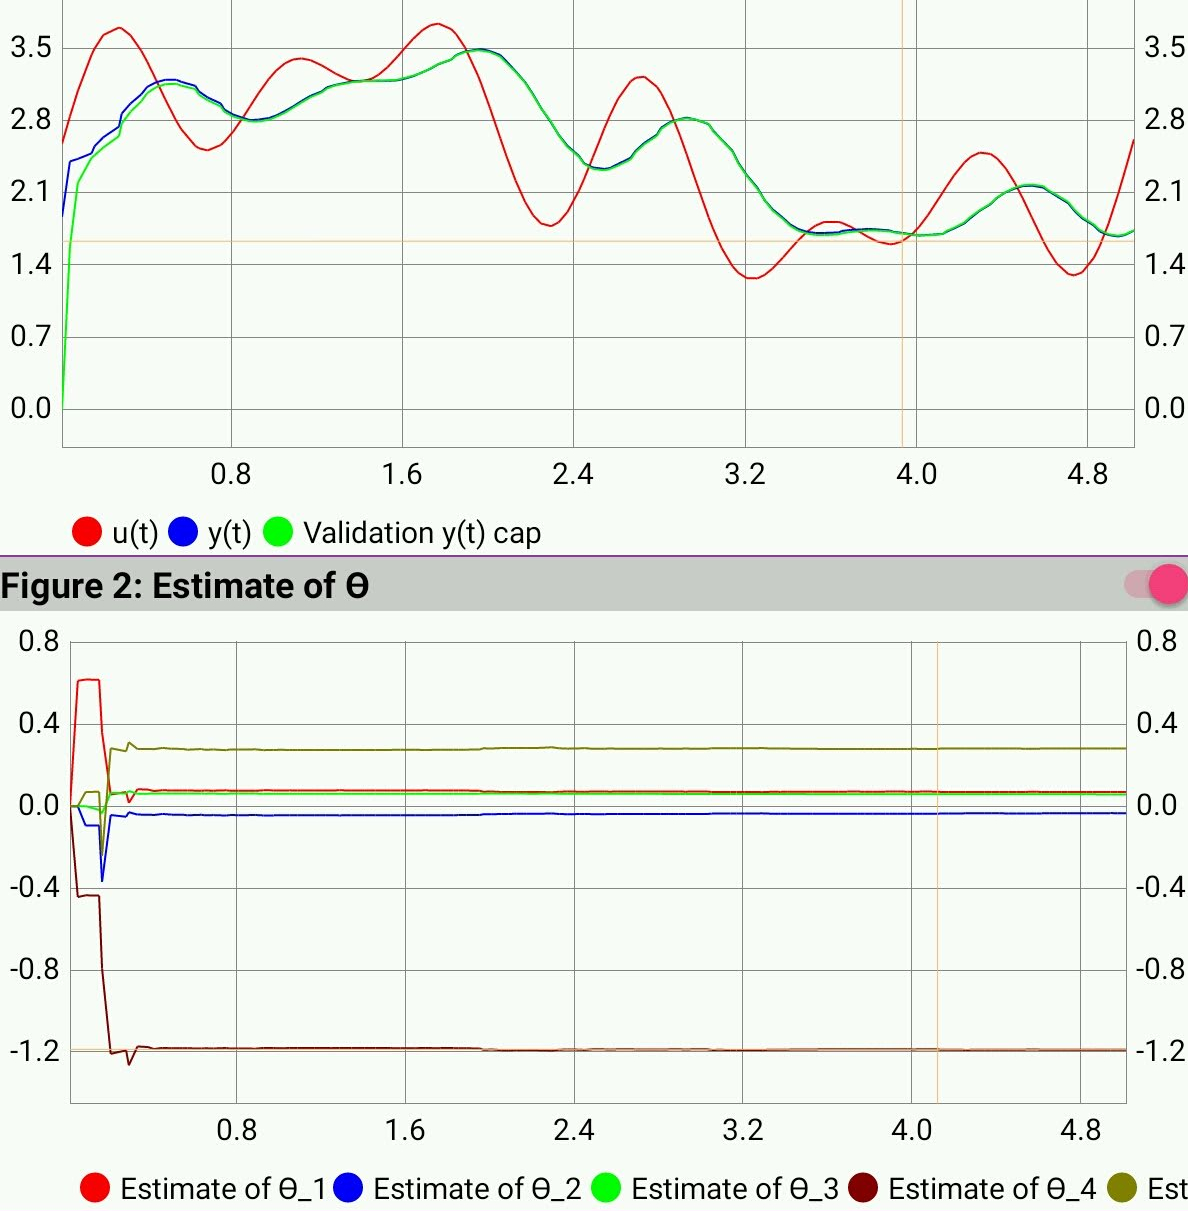
\includegraphics[width=\textwidth]{images/Fig7a-color.jpg}
	};
	\draw [FigureArrow] (-4.5,7.3) node[right] {\Large $u(t)$} -- (-5.79, 7.3);
	\draw [FigureArrow] (-4.5,6.75) node[right] {\Large $y(t)$} -- (-8.27, 6.75);
	\draw [FigureArrow] (-4.5,6.15) node[right] {\Large $\hat{y}(t)$} -- (-8.18, 6.15);
	\draw [FigureArrow] (-4.5,-1.5) node[right] {\Large $\hat\theta_1(t)$} -- (-7.75, -1.5);
	\draw [FigureArrow] (0,-1.5) node[right] {\Large $\hat\theta_5(t)$} -| (-2, -2.22);
	\draw [FigureArrow] (0,-6.2) node[right] {\Large $\hat\theta_4(t)$} -| (-2, -6.9);
	\draw [FigureArrow] (0,-4) node[right] {\Large $\hat\theta_2(t)$} -| (-2, -3.3);
	\draw [FigureArrow] (-4.5,-4) node[right] {\Large $\hat\theta_3(t)$} -| (-7.95, -3.19);

	\end{tikzpicture}
	
	\caption{Signals $u(k)$, $y(k)$, $\hat{y}(k)$ and parameters $\hat{\theta}_{1}$, $\hat{\theta}_{2}$, $\hat{\theta}_{3}$, ${{\hat{\theta }}_{4}}$ and  ${{\hat{\theta }}_{5}}$.}
	\label{Fig:SOPA_A}
\end{figure}

\begin{figure}
	\centering
	\begin{tikzpicture}[node distance = 10mm, auto]
	\node (Excitation) [align=center] {
		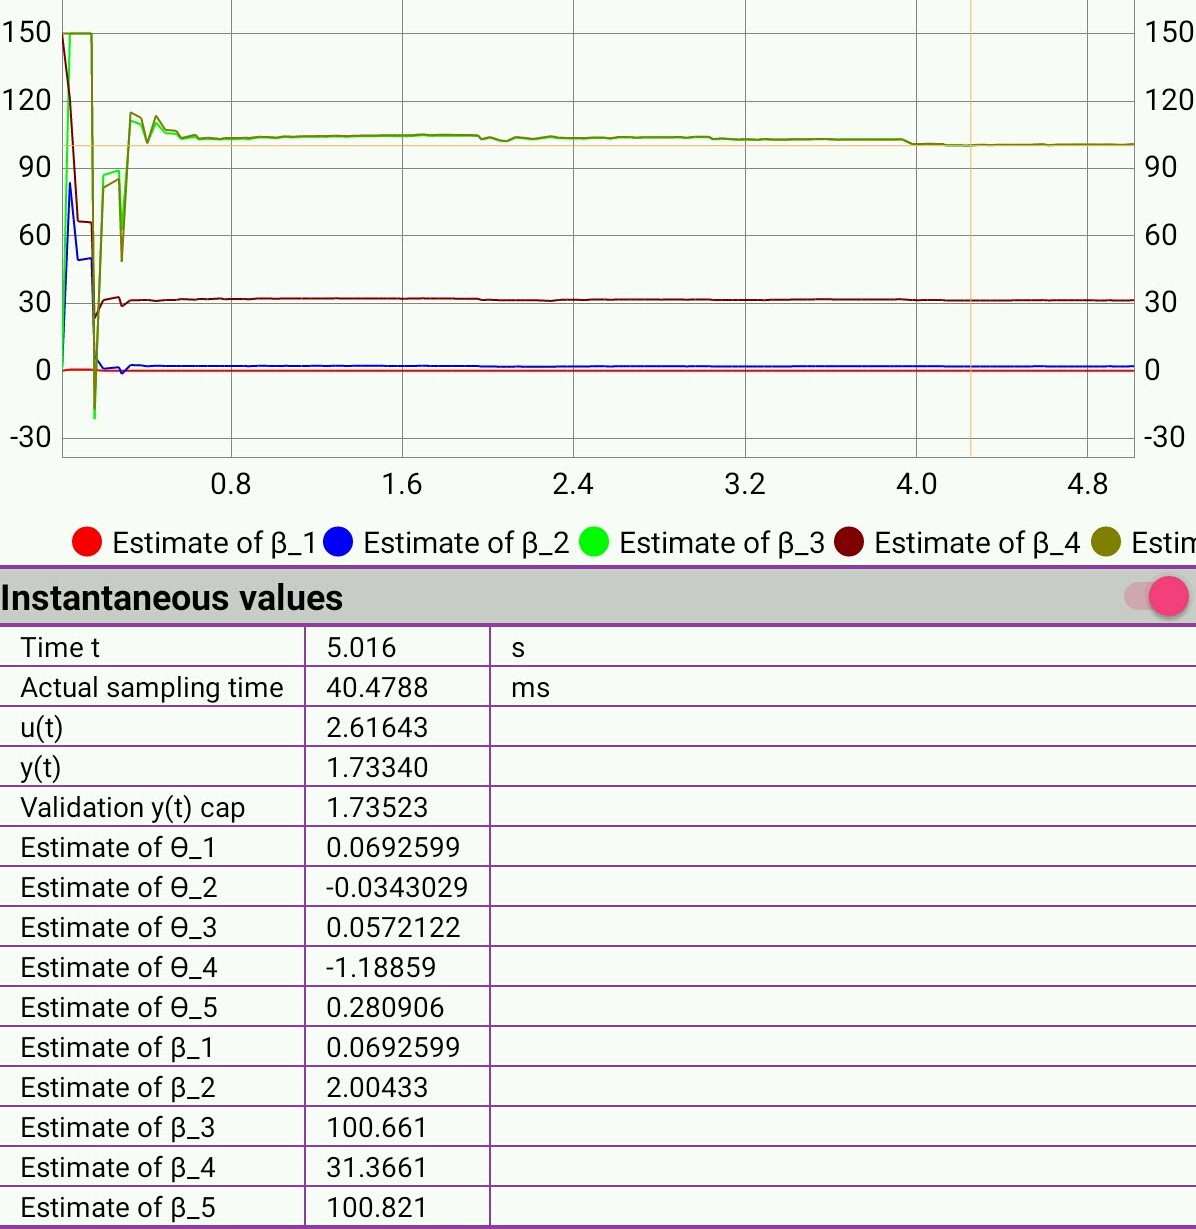
\includegraphics[width=\textwidth]{images/Fig7b-color.jpg}
	};
	\draw [FigureArrow] (-4.5,9.35) node[right] {\Large $\hat\beta_3(t)$} -| (-7.6, 6.925);
	\draw [FigureArrow] (-4.5,8.6) node[right] {\Large $\hat\beta_5(t)$} -| (-7.25, 7.8);
	\draw [FigureArrow] (-4.5,5.39) node[right] {\Large $\hat\beta_4(t)$} -| (-6.5, 4.925);
	\draw [FigureArrow] (-4.5,4.35) node[right] {\Large $\hat\beta_2(t)$} -| (-6.5, 3.885);
	\draw [FigureArrow] (-4.5,3.29) node[right] {\Large $\hat\beta_1(t)$} -| (-6.5, 3.755);
	\end{tikzpicture}
	
	\caption{Estimates $\hat{\beta}_{1}$, $\hat{\beta}_{2}$, $\hat{\beta}_{3}$, $\hat{\beta}_{4}$, $\hat{\beta}_{5}$, and instantaneous values of signals and parameters.}
	\label{Fig:SOPA_B}
\end{figure}

\begin{figure}
	\centering
	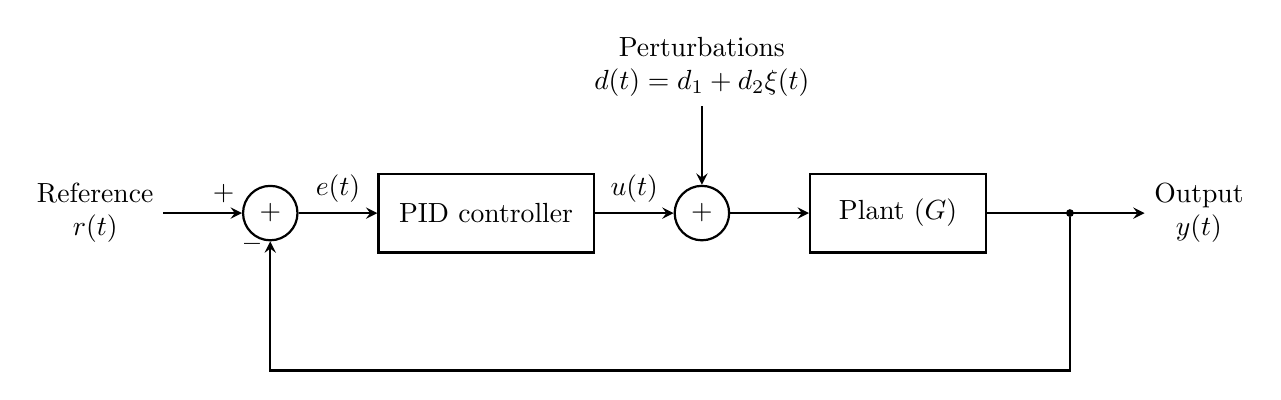
\begin{tikzpicture}[node distance = 10mm, auto]
	\node (Reference) [align=center] {Reference\\$r(t)$};
	\node (SummingPoint) [draw,circle, thick, right = of Reference]  {+};
	\node (Control) [block, text width = 2.5cm, right = of SummingPoint] {PID controller};
	\node (SummingPoint1) [draw,circle, thick, right = of Control]  {+};
	\node (Plant) [block, text width = 2cm, right = of SummingPoint1] {Plant ($G$)};
	\node (PlantRight) [support, right = of Plant, right = 1cm, fill, circle,scale=0.3] {};
	\node (Output) [right = of Plant, right = 2cm, align=center] {Output\\$y(t)$};
	\node (Perturbations) [align=center, above = of SummingPoint1] {Perturbations\\$d(t)=d_1+d_2\xi(t)$};
	\draw [arrow] (Reference) -- node[anchor=south west]{+}(SummingPoint);
	\draw [arrow] (SummingPoint) -- node[anchor=south]{$e(t)$}(Control);
	\draw [arrow] (Control) -- node[anchor=south]{$u(t)$}(SummingPoint1);
	\draw [arrow] (SummingPoint1) -- (Plant);
	\draw [arrow] (Plant) -- (Output);
	\draw [arrow] (PlantRight) -- +(0, -2) -| (SummingPoint) node[below = 2mm, anchor=north east]{\bf\textendash};
	\draw [arrow] (Perturbations) -- (SummingPoint1);
	\end{tikzpicture}
	\caption{Closed loop system with a PID Controller}
	\label{Fig:BlockDiagramPID}
\end{figure}

\begin{figure}
	\centering
	\begin{tikzpicture}[node distance = 10mm, auto]
	\node (Excitation) [align=center] {
		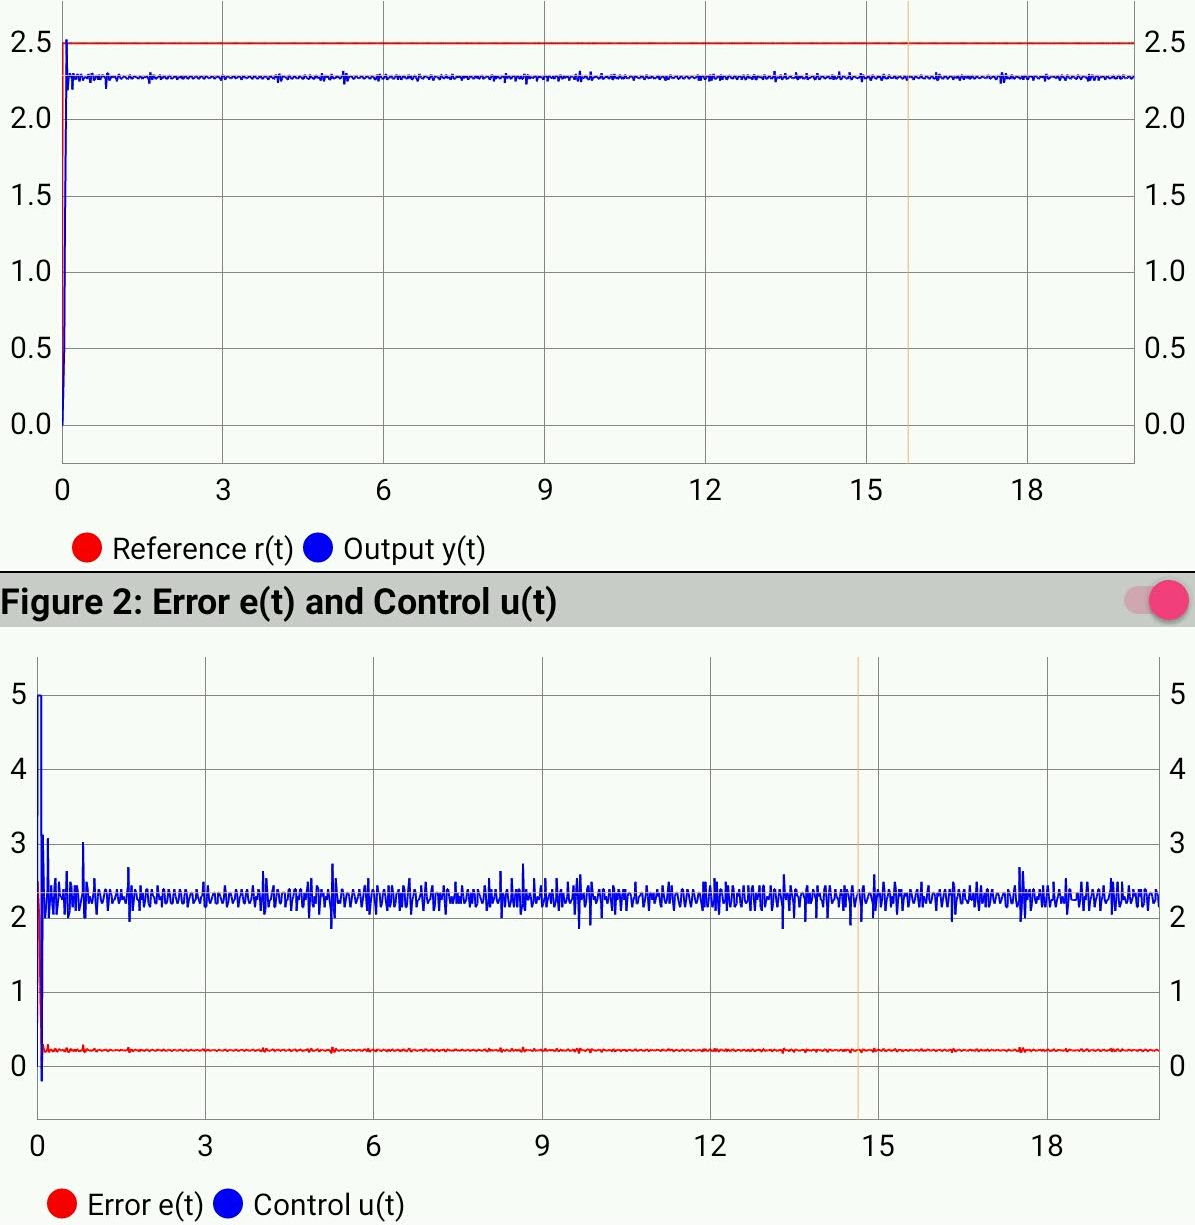
\includegraphics[width=\textwidth]{images/Fig8_cortada-color.jpg}
	};
	\draw [FigureArrow] (-4.5,7) node[right] {\Large $r(t)$} -| (-6.5, 8.84);
	\draw [FigureArrow] (-4.5,6) node[right] {\Large $y(t)$} -| (-7.5, 8.30);
	\draw [FigureArrow] (-4.5,-5.5) node[right] {\Large $u(t)$} -| (-7.5, -4.55);
	\draw [FigureArrow] (-4.5,-7.5) node[right] {\Large $e(t)$} -| (-7.5, -6.85);
	\end{tikzpicture}
	
	\caption{Signals $r(k)$, $y(k)$, $e(k)$ and $u(k)$ of the closed-loop system with ${{K}_{P}}=10$, $K_{I}=0$, and ${{K}_{D}}=0$.}
	\label{Fig:FOPID_A}
\end{figure}

\begin{figure}
	\centering
	\begin{tikzpicture}[node distance = 10mm, auto]
	\node (Excitation) [align=center] {
		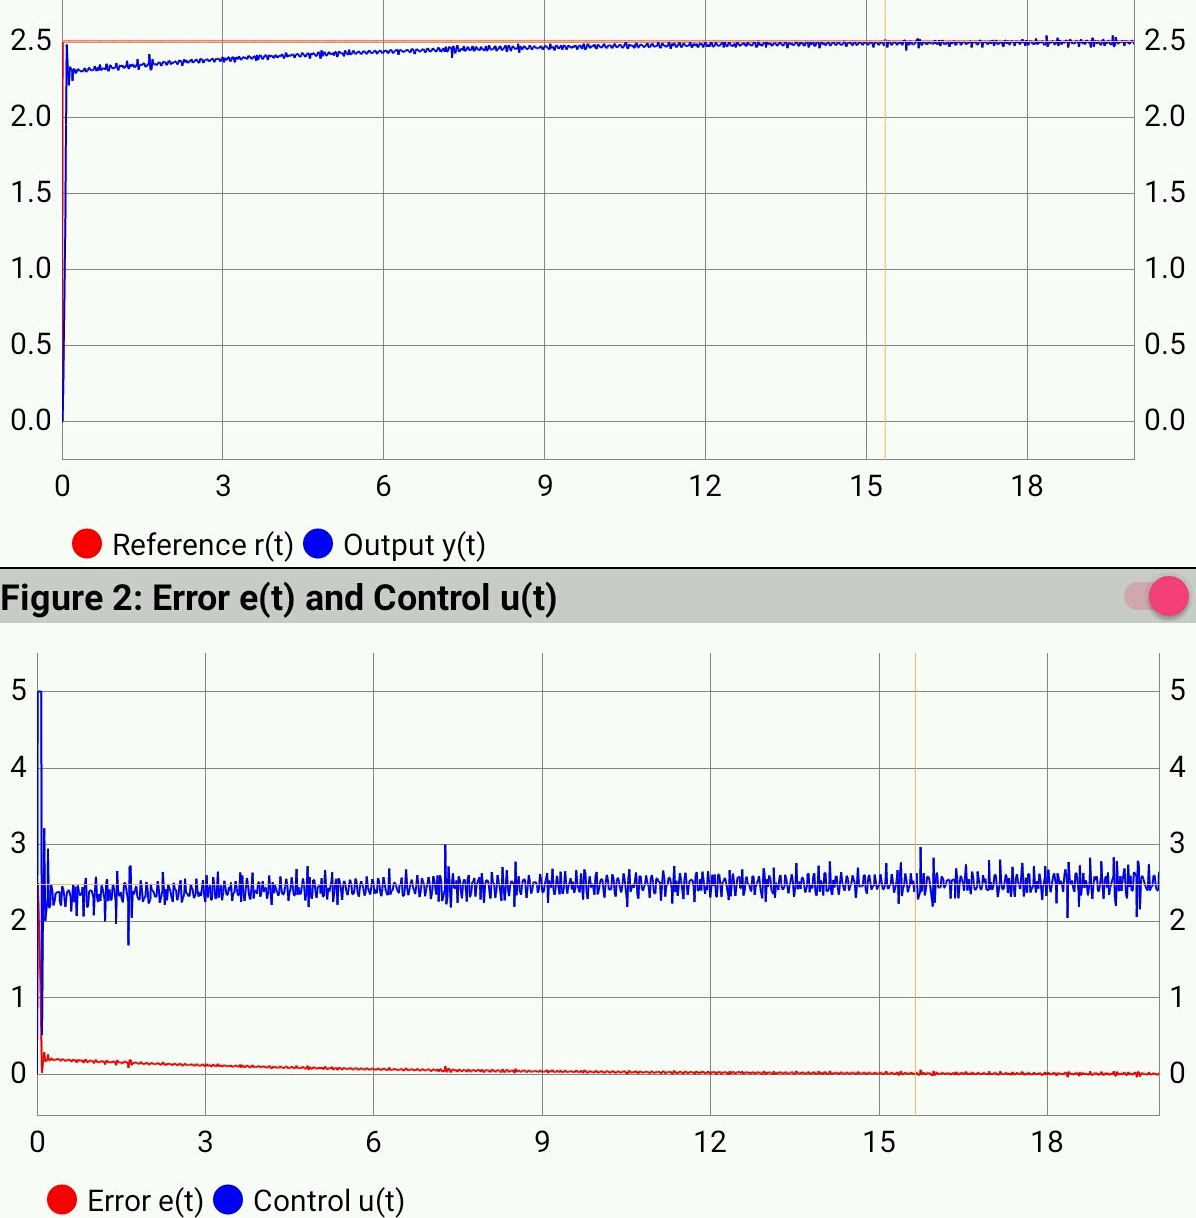
\includegraphics[width=\textwidth]{images/Fig9_cortada-color.jpg}
	};
	\draw [FigureArrow] (-4.5,7) node[right] {\Large $r(t)$} -| (-6.5, 8.80);
	\draw [FigureArrow] (-4.5,6) node[right] {\Large $y(t)$} -| (-7.5, 8.37);
	\draw [FigureArrow] (-4.5,-5.75) node[right] {\Large $u(t)$} -| (-7.36, -5.27);
	\draw [FigureArrow] (-4.5,-6.5) node[right] {\Large $e(t)$} -| (-7.36, -7);
	\end{tikzpicture}
	
	\caption{Signals $r(k)$, $y(k)$, $e(k)$ and $u(k)$ of the closed-loop system with ${{K}_{P}}=10$, ${{K}_{I}}=2$, and ${{K}_{D}}=0$.}
	\label{Fig:FOPID_B}
\end{figure}

\begin{figure}
	\centering
	\begin{tikzpicture}[node distance = 10mm, auto]
	\node (Excitation) [align=center] {
		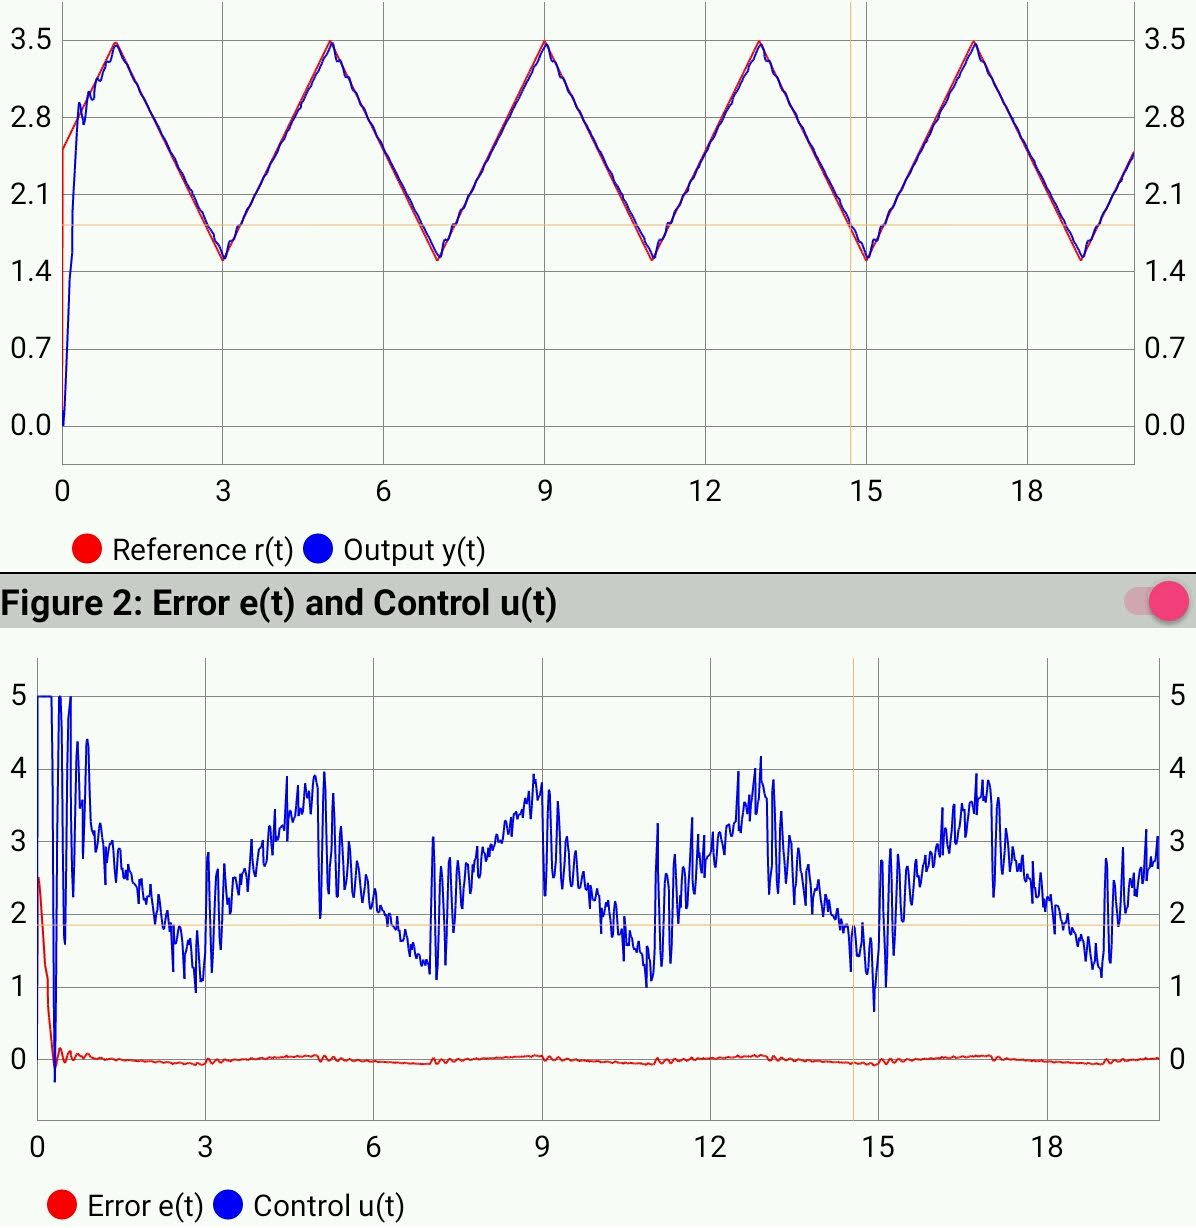
\includegraphics[width=\textwidth]{images/Fig10_cortada-color.jpg}
	};
	\draw [FigureArrow] (-4.5,9.25) node[right] {\Large $r(t)$} -| (-8.3, 7.50);
	\draw [FigureArrow] (-4.5,4.5) node[right] {\Large $y(t)$} -- (-8.28, 4.5);
	\draw [FigureArrow] (-4.5,-6.5) node[right] {\Large $u(t)$} -| (-6.315, -5.9);
	\draw [FigureArrow] (-4.5,-7.6) node[right] {\Large $e(t)$} -| (-6.315, -7.05);
	\end{tikzpicture}
	
	\caption{Signals $r(k)$, $y(k)$, $e(k)$ and $u(k)$ of the closed-loop system with ${{K}_{P}}=20$, ${{K}_{I}}=5$, and ${{K}_{D}}=0.1$.}
	\label{Fig:FOPID_C}
\end{figure}
\end{document}